\chapter{Visualizing estimation results}
\label{visualization} \index{Visualizing estimation results}

In this chapter we show, how estimation results produced with one of the regression tools described in the two previous
chapters can be visualized. In general, there are two possibilities to visualize results: Within {\em BayesX}, special
functions can be applied to regression objects. Since all three regression tools provide almost the same possibilities to
visualize results, we describe them simultaneously in the next section. Tools for the visualization of autocorrelations for
MCMC samples are described in \autoref{plotautocor}. An alternative way to visualize results is to use the R package
supplementing {\it BayesX}. Some further comments on this package are provided in \autoref{rpackage}.

\section{BayesX functions} \label{bayesxplot}

{\em BayesX} allows to visualize estimation results immediately
after estimation. The {\em output window} and/or the log file
describe how to do this for a particular model term. Nonlinear
effects of continuous covariates and time scales are plotted with
\hyperref[bayesxplotnonp]{method #plotnonp#}. Spatial effects are
visualized with \hyperref[drawmap]{method #drawmap#}. When using
{\em bayesreg objects}, autocorrelation functions of sampled
parameters can be visualized with \hyperref[plotautocor]{method
#plotautocor#}.

\newpage

\subsection{Method plotnonp} \label{bayesxplotnonp} \index{Plotting
nonparametric functions} \index{Plotnonp command}

\begin{stanza}{Description}

Method #plotnonp# is a post estimation command, i.e.~it is
meaningful only if method #regress# has been applied before. The
method allows to plot estimated effects of nonlinear covariate
effects immediately after estimation. T

\end{stanza}

\begin{stanza}{Syntax}

#># {\em objectname}.#plotnonp# {\em termnumber} [{\em , options}]


Plots the estimated effect with term number {\em termnumber}. The
term number will be printed in the {\em output window} and/or an
open log file. Several options are available for labelling axis,
adding a title, etc., see the options list below. Note that method
#plotnonp# can be applied only if random walks, P-splines or
seasonal components are used as priors.

\end{stanza}

\begin{stanza}{Options}

The following options are available for method #plotnonp# (listed
in alphabetical order):

\end{stanza}

\begin{itemize}
\item #connect=1#$|$#2#$|$#3#$|$#4#$|$#5#[{\em specifications for
further variables}]

Option #connect# specifies how points in the scatterplot are
connected. There are currently 5 different specifications:

\begin{tabular}{ll}
#1# & draw straight lines between the points (default) \\
#2#, #3#, #4# & draw dashed lines (numbers #2#-#4# indicate different variants)\\
#5# & do not connect, i.e.~plot points only \\
\end{tabular}

If you draw more than one scatterplot in the same graph (i.e. more
than one {\em yvar} is specified) you can connect points for every
{\em yvar} differently by simply specifying the corresponding
number (#1,2,3,4,5#) for every {\em yvar}. Typing for example

{\em #connect=15#}

connects the points corresponding to {\em yvar1} and {\em xvar} by
straight lines, but does not connect the points corresponding to
{\em yvar2} (if specified) and {\em xvar}. Points corresponding to
additionally specified variables $yvar3$, etc.~are connected by
straight lines.

An equivalent way of specifying the different variants is available
via the symbols #l#, #d#, #\_#, #-# and #p#, which correspond to the
numbers #1#-#5#, i.e.~

{\em #connect=12345#} is equivalent to {\em #connect=ld_-p#}

\item #fontsize = #{\em integer}

Specifies the font size (in pixels) for labelling axes etc. Note
that the title is scaled accordingly. The default is
#fontsize=12#.

\item #height = #{\em integer}

Specifies the height (in pixels) of the graph. The default is
#height=210#.

\item #levels = all#$|$#1#$|$#2#$|$#none#

By default, #plotnonp# plots the estimated nonlinear covariate
effect together with the pointwise credible intervals based on
nominal levels of 80\% and 95\% (the nominal levels may be changed
using the options \hyperref[level1]{level1} and/or
\hyperref[level2]{level2}). Option #levels# allows to omit
completely pointwise credible intervals in the graphs
(#levels=none#), print only the 95\% credible intervals
(#levels=1#) or to print only the 80\% credible intervals
(#levels=2#).

 \item #linecolor = B#$|$#b#$|$#c#$|$#G#$|$#g#$|$#o#$|$#m#$|$#r#$|$#y# [{\em specifications for further
variables}]

Option #linecolor# specifies the color to be used for drawing
lines (or points, see option #connect#) in the scatterplot.
Currently the following specifications are available:

\begin{tabular}{ll}
#B# & black (default) \\
#b# & blue \\
#c# & cyan \\
#G# & gray \\
#g# & green \\
#o# & orange \\
#m# & magenta \\
#r# & red \\
#y# & yellow
\end{tabular}

If you draw more than one scatterplot in the same graph (i.e. more
than one {\em yvar} is specified) you can use different colors for
each {\em yvar} by simply specifying the corresponding symbol
(#B,b,c,G,g,o,m,r,y#) for each {\em yvar}. Typing for example

{\em #linecolor = Bgr#}

colors the lines (points) corresponding to {\em yvar1} and {\em
xvar} in black, whereas the points corresponding to {\em yvar2}
and {\em yvar3} (if specified) and {\em xvar} are colored in green
and red, respectively.

\item #linewidth = #{\em integer}

Specifies how thick lines should be drawn. The default is
#linewidth=5#.

\item #outfile = #{\em characterstring}

If option #outfile# is specified the graph will be stored as a
postscript file rather than being printed on the screen. The path
and the filename must be specified in {\em characterstring}. By
default, an error will be raised if the specified file is already
existing or the specified folder is not existing. To overwrite  an
already existing file, option #replace# must be additionally
specified. This prevents you from unintentionally overwriting your
files.

\item #pointsize = #{\em integer}

Specifies the size of the points (in pixels) if drawing points
rather than lines is specified. The default is #pointsize=20#.

\item #replace#

The #replace# option is useful only in combination with option
#outfile#. Specifying #replace# as an additional option allows the
program to overwrite an already existing file (specified in
#outfile#), otherwise an error will be raised.

\item #title = #{\em characterstring}

Adds a title to the graph. If the title contains more than one
word, {\em characterstring} must be enclosed by quotation marks
(e.g. \texttt{title="my first title"}).

\item #titlesize = #{\em realvalue}

Specifies the factor by which the size of the title is scaled
relative to the size of the labels of the axes (compare option
#fontsize#). The default is \texttt{titlesize=1.5}.

\item #width = #{\em integer}

Specifies the width (in pixels) of the graph. The default is
#width=356#.

\item #xlab = #{\em characterstring}

Labels the x-axis. If the label contains more than one word, {\em
characterstring} must be enclosed by quotation marks (e.g.
\texttt{xlab="x axis"}).

\item #xlimbottom = #{\em realvalue}

Specifies the minimum value at the x-axis to be plotted. The
default is the minimum value in the data set. If #xlimbottom# is
above the minimum value in the data set, only a part of the graph
will be visible.

\item #xlimtop = #{\em realvalue}

Specifies the maximum value at the x-axis to be plotted. The
default is the maximum value in the data set. If #xlimtop# is
below the maximum value in the data set, only a part of the graph
will be visible.

\item #xstart = #{\em realvalue}

Specifies the value where the first 'tick' on the x-axis should be
drawn. The default is the minimum value on the x-axis.

\item #xstep = #{\em realvalue}

If #xstep# is specified,  ticks are drawn at the x-axis with
stepwidth {\em realvalue} starting at the minimum value on the
x-axis (or at the value specified in option #xstart#). By default,
five equally spaced ticks are drawn at the x-axis.

\item #ylab = #{\em characterstring}

Labels the y-axis. If the label contains more than one word, {\em
characterstring} must be enclosed by quotation marks (e.g.
\texttt{ylab="y axis"}).

\item #ylimbottom = #{\em realvalue}

Specifies the minimum value at the y-axis to be plotted. The
default is the minimum value in the data set. If #ylimbottom# is
above the minimum value in the data set, only a part of the graph
will be visible.

\item #ylimtop = #{\em realvalue}

Specifies the maximum value at the y-axis to be plotted. The
default is the maximum value in the data set. If #ylimtop# is
below the maximum value in the data set, only a part of the graph
will be visible.

\item #ystart = #{\em realvalue}

Specifies the value where the first 'tick' on the y-axis should be
drawn. The default is the minimum value on the y-axis.

\item #ystep = #{\em realvalue}

If #ystep# is specified,  ticks are drawn at the y-axis with
stepwidth {\em realvalue} starting at the minimum value on the
y-axis (or at the value specified in option #ystart#). By default,
five equally spaced ticks are drawn at the y-axis.
\end{itemize}

\newpage

\begin{stanza}{Examples}

Suppose we have already created a regression object #reg# and have
estimated a regression model with Gaussian errors using a command
like

#> reg.regress Y = X(psplinerw2), family=gaussian using d#

where #Y# is the response variable and #X# the only explanatory
variable. The effect of #X# is modelled nonparametrically using
Bayesian P-splines. In the {\em output window} we obtain the
following estimation output for the effect of #X#:

\begin{verbatim}
  f_x

  Results are stored in file
  c:\results\reg_f_x_pspline.res
  Results may be visualized using method plotnonp
  Type for example: objectname.plotnonp 0
\end{verbatim}

The term number of the effect of X is 0, i.e. by typing

#> reg.plotnonp 0#

we obtain the plot shown in \autoref{plotnonpexample1}.

Of course, a title, axis labels etc. can be added. For example by
typing

#> reg.plotnonp 0 , title="my title" xlab="x axis"#

we obtain the plot shown in \autoref{plotnonpexample2}.

By default, the plots appear in an additional window on the
screen. They can be directly stored in postscript format by adding
option #outfile#. For example by typing

 #> reg.plotnonp 0 , title="my title" xlab="x axis" outfile="c:\results\result1.ps"#

the graph is stored in postscript format in the file
#c:\results\result1.ps#.


\begin{figure}[p]
\begin{center}
\includegraphics[scale=0.8]{grafiken/plotnonpexample.ps}
{\em\caption{ \label{plotnonpexample1} Illustration for the usage of
method \em\tt plotnonp}}
\end{center}
\end{figure}


\begin{figure}[p]
\begin{center}
\includegraphics[scale=0.8]{grafiken/plotnonpexample2.ps}
{\em\caption{ \label{plotnonpexample2} Second illustration for the
usage of method \em\tt plotnonp}}
\end{center}
\end{figure}

\end{stanza}

\clearpage

\subsection{Method drawmap} \label{drawmap}
\index{Drawmap command}

\begin{stanza}{Description}

Method #drawmap# is a post estimation command, i.e.~it is meaningful
only if method #regress# has been applied before. The method allows
to visualize estimated effects of spatial covariates immediately
after estimation.

\end{stanza}

\begin{stanza}{Syntax}

#># {\em objectname}.#drawmap# {\em termnumber} [{\em , options}]

Visualizes the effect of a spatial covariate by coloring the
regions of the corresponding geographical map according to the
estimated effect (or other characteristics of the posterior). The
term number {\em termnumber} identifies the model term and can be
found in the {\em output window} and/or an open log file. Several
options are available for adding a title or changing the color
scale etc., see the options list below. Note that method #drawmap#
can be applied only if Markov random fields, geosplines or
geokriging are used as priors.

\end{stanza}

\begin{stanza}{Options}

The following options are available for method #drawmap# (in
alphabetical order):

\end{stanza}

\begin{itemize}
\item #color#

The #color# option allows to choose between a grey scale for the
colors and a colored scale. If #color# is specified a colored
scale is used instead of a grey scale.

\item #drawnames#

In some situations it may be useful to print the names of the
regions into the graph (although the result may be confusing in
most cases). This can be done by specifying the additional option
#drawnames#. By default the names of the regions are omitted in
the map.

\item #fontsize = #{\em integer}

Specifies the font size (in pixels) for labelling the legend and
writing the names of the regions (if specified). Note, that the
title is scaled accordingly (see option #titlesize#). The default is
#fontsize=12#.

\item #hcl#

Requests that a color palette from the HCL color space should be
used instead of an RGB palette. The HCL colors will be selected
diverging from a neutral center (grey) to two different extreme
colors (red and green) in contrast to the RGB colors diverging from
yellow to red and green. HCL colors are particularly useful for
electronic presentations since they are device-independent. The
option #hcl# is only meaningful in combination with the option
#color#.

\item #lowerlimit = #{\em realvalue}

Lower limit of the range to be drawn. If #lowerlimit# is omitted,
the minimum numerical value in #plotvar# will be used instead as
the lower limit.

\item #nolegend#

By default a legend is drawn into the graph. By specifying the
option #nolegend# the legend will be omitted.

\item #nrcolors = #{\em integer}

To color the regions according to their numerical characteristics,
the data are divided into a (typically large) number of ordered
categories. Afterwards a color is associated with each category. The
#nrcolors# option can be used to specify the number of categories
(and with it the number of different colors). The maximum number of
colors is 256, which is also the default value.

\item #outfile = #{\em characterstring}

If option #outfile# is specified the graph will be stored as a
postscript file rather than being printed on the screen. The path
and the filename must be specified in {\em characterstring}. By
default, an error will be raised if the specified file is already
existing or the specified folder is not existing. To overwrite an
already existing file, option #replace# must be additionally
specified. This prevents you from unintentionally overwriting your
files.

\item #pcat#

If you want to visualize the values of the columns #pcat80# or
#pcat95# it is convenient to specify #pcat#. This forces #drawmap#
to expect a column that consists only of the values -1, 0 and 1. Of
course you can achieve the same result by setting #nrcolors=3#,
#lowerlimit=-1# and #upperlimit=1#.

\item #plotvar = #{\em variablename}

By default, the regions of the map are colored according to the
estimated spatial effect. Option #plotvar# allows to color the map
according to other characteristics of the posterior by explicitly
specifying the name of the variable to be plotted. Compare the
header of the file containing the estimation results to see all
variables available for plotting.

\item #replace#

The #replace# option is only useful in combination with option
#outfile#. Specifying #replace# as an additional option allows the
program to overwrite an already existing file (specified in
#outfile#), otherwise an error will be raised.

\item #swapcolors#

In some situations it may be favorable to swap the order of the
colors, i.e.~black (red) shades corresponding to large values and
white (green) shades corresponding to small values. This is
achieved by specifying #swapcolors#. By default, small values are
colored in black shades (red shades) and large values in white
shades (green shades).

\item #title = #{\em characterstring}

Adds a title to the graph. If the title contains more than one
word, {\em characterstring} must be enclosed by quotation marks
(e.g. #title="my first map"#).

\item #titlesize = #{\em realvalue}

Specifies the factor by which the size of the title is scaled
relative to the size of the labels of the legend (compare option
#fontsize#). The default is \texttt{titlesize=1.5}.

\item #upperlimit = #{\em realvalue}

Upper limit of the range to be plotted. If #upperlimit# is
omitted, the maximum numerical value in #plotvar# will be used
instead as the upper limit.

\end{itemize}

\newpage

\begin{stanza}{Examples}

Suppose we have already created a regression object #reg# and have
estimated a regression model with Gaussian errors using something
like

#> map m# \\
#> m.infile using c:\maps\map1.bnd#

#> reg.regress Y = region(spatial,map=m), family=gaussian using d#

where #Y# is the response variable and #region# the only
explanatory variable. The effect of the spatial covariate #region#
is modelled nonparametrically  using a Markov random field. In the
{\em output window} we obtain the following estimation output for
the effect of #region#:

\begin{verbatim}
  f_spat_region

  Results are stored in file
  c:\results\reg_f_region_spatial.res
  Results may be visualized using method 'drawmap'
  Type for example: objectname.drawmap 0
\end{verbatim}

The term number of the effect of #region# is 0, i.e.~by typing

#> reg.drawmap 0#

we obtain the map shown in \autoref{drawmapexample1} where the
regions are colored according to the estimated spatial effect.

By default the regions are colored in grey scale. A color scale is
obtained by adding option #color#. A title can be added as well.
For example by typing

#> reg.drawmap 0 , color title="my title"#

we obtain the map shown in \autoref{drawmapexample2}.

By default, the maps appear in an additional window on the screen.
They can be directly stored in postscript format by adding option
#outfile#. For example by typing

 #> reg.drawmap 0 , color title="my title" outfile="c:\results\result1.ps"#

the colored map is stored in postscript format in the file
#c:\results\result1.ps#.

\begin{figure}[ht]
\begin{center}
\includegraphics[scale=0.4]{grafiken/drawmapexample.ps}
{\em\caption{ \label{drawmapexample1} Illustration for the usage
of method \em \texttt{drawmap}}}
\end{center}
\end{figure}


\begin{figure}[ht]
\begin{center}
\includegraphics[scale=0.4]{grafiken/drawmapexample2.ps}
{\em\caption{ \label{drawmapexample2} Second illustration for the
usage of method \em \texttt{drawmap}}}
\end{center}
\end{figure}

\end{stanza}

\clearpage

\subsection{Method plotautocor} \label{plotautocor}
\index{Plotautocor command}

\begin{stanza}{Description}

Method #plotautocor# is a post estimation command, i.e.~it is
meaningful only if method #regress# has been applied before.
Method #plotautocor# computes and visualizes the autocorrelation
functions of the parameters in the model. This method is only
applicable to {\em bayesreg objects}.

\end{stanza}

\begin{stanza}{Syntax}

#># {\em objectname}.#plotautocor# [{\em , options}]

Computes and visualizes the autocorrelation functions in the
model. Several options are available for specifying the maximum
lag for autocorrelations, storing the graphs in postscript format
etc., see the options list below.

\end{stanza}

\begin{stanza}{Options}

The following options are available for method #plotautocor# (in
alphabetical order):

\end{stanza}

\begin{itemize}
\item #maxlag = #{\em integer}

Option #maxlag# may be used to specify the maximum lag for
autocorrelations. The default is #maxlag=250#.

\item #mean#

If option #mean# is specified, for each lag number and model term
only minimum, mean and maximum autocorrelations are plotted. This
can lead to a considerable reduction in computing time and storing
size.

\item #outfile = #{\em characterstring}

If option #outfile# is specified the graph will be stored as a
postscript file and not printed on the screen. The path and the
filename must be specified in {\em characterstring}. An error will
be raised if the specified file is already existing and the
#replace# option is not specified.

\item #replace#

The #replace# option is only useful in combination with option
#outfile#. Specifying #replace# as an additional option allows the
program to overwrite an already existing file (specified in
#outfile#), otherwise an error will be raised.
\end{itemize}

\begin{stanza}{Examples}

Suppose we have already created a {\em bayesreg object} #reg# and
have estimated a regression model with Gaussian errors using

#> reg.regress Y = X(psplinerw2), family=gaussian using d#

where #Y# is the response variable and #X# the only explanatory
variable. The effect of #X# is modelled nonparametrically  using
Bayesian P-splines. We can now check the mixing of sampled
parameters by computing and drawing the autocorrelation functions
up to a maximum lag of 150:

#> reg.plotautocor , maxlag=150 outfile="c:\results\autocor.ps"#

In this example the autocorrelation functions are not shown on the
screen but stored in postscript format in the file
#c:\results\autocor.ps#. If option #outfile# is omitted, the
functions are plotted on the screen. The resulting file contains 5
pages. As an example, the first page of the file is shown in
\autoref{autocorexample}.

\begin{figure}[ht]
\begin{center}
\includegraphics[scale=0.8]{grafiken/autocorexample1.ps}
{\em\caption{ \label{autocorexample} Illustration for the usage of
method \em\texttt{plotautocor}}}
\end{center}
\end{figure}

\end{stanza}

\clearpage

\section{R package BayesX}\label{rpackage} \index{R} \index{R package}

To provide some convenient graphics facilities for the command line version of {\it BayesX}, an R package has been developed
that contains virtually the same functionality as described in the preceding section. In addition, routines for manipulating
geographical information are available. The R package {\it BayesX} is available from CRAN
(\href{http://www.r-project.org}{http://www.r-project.org}).
